\documentclass[utf8x,xcolor=pdftex,dvipsnames,table]{beamer}
\usetheme{Malmoe}  % Now it's a beamer presentation with the lisa theme!
\setbeamertemplate{footline}[page number]
\usecolortheme{beaver}
\usepackage[T1]{fontenc}
\usepackage{amsmath}
\usepackage[utf8x]{inputenc}
\usepackage{multicol}
%\logo{
\includegraphics[width=.8in]{UdeM_NoirBleu_logo_Marie_crop}}
\usepackage{listings}
\usepackage{tikz}

\newcommand{\superscript}[1]{\ensuremath{^{\textrm{#1}}}}

\mode<presentation>

\title{Instructor-Led Lab: Image Classification using the Theano Python Library}

\author{%
\footnotesize
Frédéric Bastien \newline
\newline
\newline
Montreal Institute for Learning Algorithms \newline
Université de Montréal \newline
Montréal, Canada \newline
\texttt{bastienf@iro.umontreal.ca} \newline \newline
Presentation prepared with Pierre Luc Carrier and Arnaud Bergeron
}

\date{GTC 2017}

\setbeamertemplate{navigation symbols}{}
\begin{document}

\begin{frame}[plain]
 \titlepage
 \vspace{-5em}
 
\includegraphics[width=1.4in]{pics/MILA.png}
 \hfill
 
\includegraphics[width=.8in]{pics/UdeM_NoirBleu_logo_Marie_crop}
\end{frame}

\section{LABS}

{ % all template changes are local to this group.
  \setbeamertemplate{navigation symbols}{}
  \begin{frame}[plain]
    \begin{tikzpicture}[remember picture,overlay]
      \node[at=(current page.center)] {
        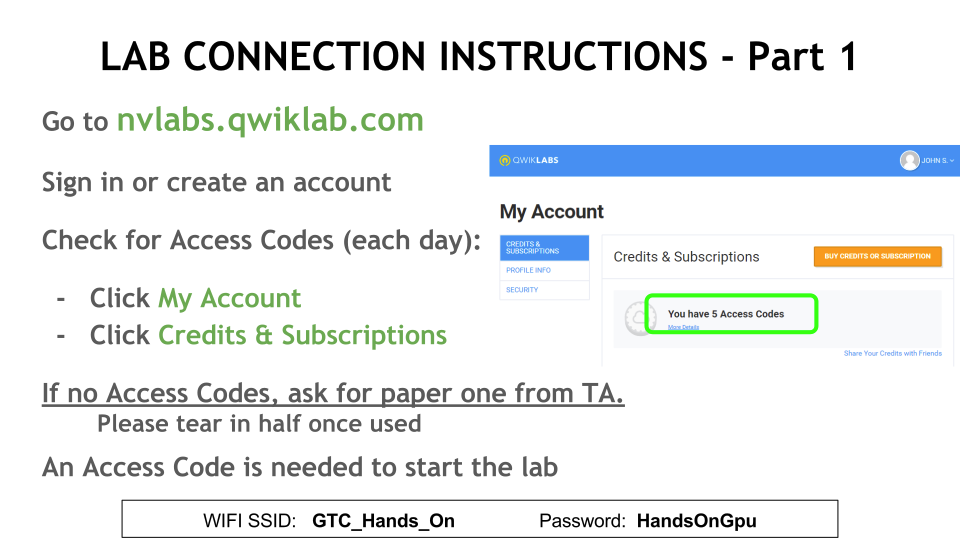
\includegraphics[width=\paperwidth]{pics/Intro_Lab_Slides1.png}
      };
    \end{tikzpicture}
  \end{frame}
  \begin{frame}[plain]
    \begin{tikzpicture}[remember picture,overlay]
      \node[at=(current page.center)] {
        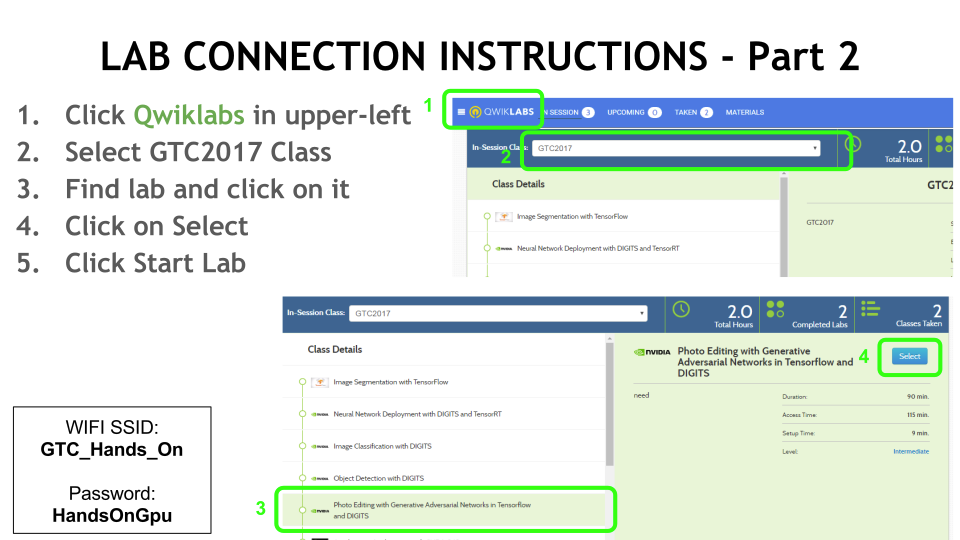
\includegraphics[width=\paperwidth]{pics/Intro_Lab_Slides2.png}
      };
    \end{tikzpicture}
  \end{frame}
}

\begin{frame}{Slides}
\begin{itemize}
% \item PDF of the slides: \url{https://goo.gl/z0tynd}
 \item github repo of this presentation \url{https://github.com/nouiz/gtc2017/}
\end{itemize}
\end{frame}

\section{Introduction}
\begin{frame}
  \tableofcontents[currentsection]
\end{frame}

\begin{frame}{High level}\setcounter{page}{1}
  Python <- \{NumPy/SciPy/libgpuarray\} <- Theano <- \{...\}
  \begin{itemize}
  \item Python: OO coding language
  \item Numpy: $n$-dimensional array object and scientific computing toolbox
  \item SciPy: sparse matrix objects and more scientific computing functionality
  \item libgpuarray: GPU $n$-dimensional array object in C for CUDA and OpenCL(not ready!)
  \item Theano: compiler/symbolic graph manipulation
    \begin{itemize}
    \item \bf{(Not a machine learning framework/software)}
    \end{itemize}
  \item \{...\}: Many libraries built on top of Theano
  \end{itemize}
\end{frame}

\begin{frame}{What Theano provides}
  \begin{itemize}
    \item Lazy evaluation for performance
    \item GPU support
    \item Symbolic differentiation
    \item Automatic speed and stability optimization
  \end{itemize}

\end{frame}

\begin{frame}{High level}
  Many [machine learning] library build on top of Theano
  \begin{itemize}
  \item Keras
  \item lasagne
  \item PyMC 3
  \item blocks
  \item sklearn-theano
  \item theano-rnn
  \item Morb
  \item ...
  \end{itemize}
\end{frame}

\begin{frame}{Goal of the stack}
\begin{center}
\begin{bf}Fast to develop\end{bf}\newline \bigskip
\begin{bf}Fast to run\end{bf}\newline \bigskip
\hspace{-2.5cm}
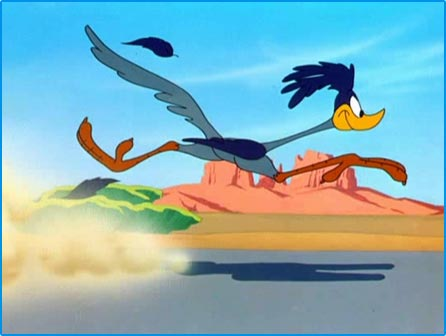
\includegraphics[width=0.35\textwidth]{pics/road-runner-1.jpg}
\end{center}
\end{frame}

\begin{frame}{Some models build with Theano}
  Some models that have been build with Theano.
  % TODO updates!resnet, NiN, memory model
  % Inception a particular case of NiN? similar idea?
  \begin{itemize}
  \item Neural Networks
  \item Convolutional NN: CNN, AlexNet, OverFeat, GoogLeNet, Inception, UNet, ...
  \item Recurrent NN: RNN, CTC, LSTM, GRU, attention mechanisms, ...
  \item NADE, RNADE, MADE
  \item Autoencoders: AE, VAE, ...
  \item Generative Adversarial Nets
  \item SVMs
  \item \begin{bf}many variations of above models and more\end{bf}
  \end{itemize}
\end{frame}

%% \begin{frame}{Others}
%%   \begin{itemize}
%%   \item IPython: Advanced python shell
%%   \item IPython notebook: web-based interactive computational environment where you can combine code execution, text, mathematics, plots and rich media into a single document
%%   \item matplotlib: one of the many plotting library
%%  \item PyTables: hdf5 container with extra functionality
%%  \item pandas: other data structure
%%  \item ...
%%   \end{itemize}
%% \end{frame}

\begin{frame}{Project status}
  \begin{itemize}
    \item Mature: Theano has been developed and used since January 2008 (9 yrs old)
    \item Driven hundreds of research papers % Over a thousands of research paper
    \item Good user documentation
    \item Active mailing list with worldwide participants
    \item Core technology for Silicon-Valley start-ups
    \item Many contributors (some from outside our institute)
    \item Used to teach many university classes
    \item Used for research at big compagnies
    \item Theano 0.9 released 20th of March, 2017
  \end{itemize}
  Theano: \url{deeplearning.net/software/theano/}

  Deep Learning Tutorials: \url{deeplearning.net/tutorial/}
\end{frame}

\subsection{Community}
\begin{frame}{Theano community}
Active community
  \begin{itemize}
  \item Many people reply on our mailing lists
  \item Hundreds of answered questions on StackOverflow
  \item 123 contributors to Theano 0.9
  \item Main developers at MILA
  \end{itemize}
\end{frame}

%% \begin{frame}{MILA}
%% Institut des algorithmes d'apprentissage de Montréal\newline
%% Montreal Institute for Machine Learning\newline
%% \begin{itemize}
%% \item Professors 8
%% \item Staff 11
%% \item Visiting Scientists 1
%% \item Post-Doc 9
%% \item Ph.D. students 46
%% \item M.Sc. students 23
%% \item Interns 15
%% \item Total 113
%% \end{itemize}
%%  \vspace{-5em}
%%  \hspace{19em}
%%  
\includegraphics[width=1.4in]{pics/MILA.png}
%%  \hfill
%% \url{mila.umontreal.ca} \newline
%% \end{frame}

%% \begin{frame}{MILA Partners}
%%     \begin{multicols}{2}
%%   \begin{itemize}

%% \item Many universities
%% \item NVIDIA
%% \item Nuance
%% \item IBM
%% \item Google
%% \item Facebook
%% \item Huawei
%% \item amazon.com
%% \item Druide
%% \item Microsoft
%% \item Intel
%% \item D-Wave
%% \item ApSTAT
%% \item Qualcomm
%% \item Imagia
%% \item Sulfur Heron
%% \item Ubisoft
%%     \end{itemize}

%% \end{multicols}
%% \end{frame}

\begin{frame}{Python}
  \begin{itemize}
  \item General-purpose high-level OO interpreted language
  \item Emphasizes code readability
  \item Comprehensive standard library
  \item Dynamic type and memory management
  \item Easily extensible with C
  \item Slow execution
  \item Popular in {\em web development}\ and {\em scientific communities}
  \end{itemize}
\end{frame}

\begin{frame}{NumPy/SciPy}
  \begin{itemize}
%  \item Python floats are full-fledged objects on the heap
%      \begin{itemize}
%      \item Not suitable for high-performance computing!
%      \end{itemize}

  \item NumPy provides an $n$-dimensional numeric array in Python
      \begin{itemize}
      \item Perfect for high-performance computing
      \item Slices of arrays are views (no copying)
      \end{itemize}

  \item NumPy provides
      \begin{itemize}
      \item Elementwise computations
      \item Linear algebra, Fourier transforms
      \item Pseudorandom number generators (many distributions)
      \end{itemize}

  \item SciPy provides lots more, including
      \begin{itemize}
      \item Sparse matrices
      \item More linear algebra
      \item Solvers and optimization algorithms
      \item Matlab-compatible I/O
      \item I/O and signal processing for images and audio
      \end{itemize}
  \end{itemize}
\end{frame}

\section{Theano}
\begin{frame}
  \tableofcontents[currentsection]
\end{frame}

%\subsection{Introduction}
\begin{frame}{Description}

  High-level domain-specific language for numeric computation.

  \begin{itemize}
    \item \begin{bf}Syntax as close to NumPy\end{bf} as possible
    \item \begin{bf}Compiles\end{bf} most common expressions \begin{bf}to C for CPU and/or GPU\end{bf}
    \item \begin{bf}Limited expressivity\end{bf} means more opportunities for optimizations
    \begin{itemize}
      \item \begin{bf}Strongly typed\end{bf} -> compiles to C
      \item \begin{bf}Array oriented\end{bf} -> easy parallelism
      \item Support for \begin{bf}looping and branching\end{bf} in expressions
      \item No subroutines -> \begin{bf}global optimization\end{bf}
    \end{itemize}
    \item \begin{bf}Automatic\end{bf} speed and numerical stability \begin{bf}optimizations\end{bf}
  \end{itemize}
\end{frame}

\begin{frame}{Description (2)}

  \begin{itemize}
    \item \begin{bf}Symbolic differentiation and R op\end{bf} (Hessian Free Optimization)
    \item Can \begin{bf}reuse other technologies\end{bf} for best performance
    \begin{itemize}
      \item CUDA, CuBLAS, CuDNN, BLAS, SciPy, PyCUDA, Cython, Numba, ...
    \end{itemize}
    \item Works on \begin{bf}Linux, OS X and Windows\end{bf}
    \item \begin{bf}Multi-GPU\end{bf} (via platoon)
    \item New GPU back-end:
      \begin{itemize}
      \item \begin{bf}Float16 storage\end{bf} new back-end (need cuda 7.5)
      \item \begin{bf}Multi dtypes\end{bf}
      \item \begin{bf}Much simpler installation on Windows\end{bf}
%      \item Multi-GPU support in the same process
      \end{itemize}
%    \item Sparse matrices (CPU only)
    \item Extensive unit-testing and self-verification
    \item Extensible (You can create new operations as needed)
  \end{itemize}
\end{frame}



%% \begin{frame}{Why scripting for GPUs?}
%%   \begin{bf}They complement each other\end{bf}

%%   GPUs are everything that high level languages are not

%%   \begin{itemize}
%%     \item Highly parallel
%%     \item Very architecture-sensitive
%%     \item Built for maximum FP/memory throughput
%%     \item So hard to program that meta-programming is easier
%%   \end{itemize}

%%   \begin{bf}Best of both worlds:\end{bf} easily scripted code which invokes high-performance GPU kernels.

%%   \begin{bf}Theano C code generation removes overhead\end{bf} of
%%   function calls between Python and C by launching many C functions at once.

%% \end{frame}

%\subsection{Simple Example}
\begin{frame}[fragile]
  \frametitle{Simple example}

\lstset{language=Python,
        commentstyle=\itshape\color{blue},
        stringstyle=\color{violet},
        }
\begin{lstlisting}
import theano
# declare symbolic variable
a = theano.tensor.vector("a")

# build symbolic expression
b = a + a ** 10

# compile function
f = theano.function([a], b)

# Execute with numerical value
print f([0, 1, 2])
# prints `array([0, 2, 1026])`
\end{lstlisting}
\end{frame}

\begin{frame}{Simple example}
\center
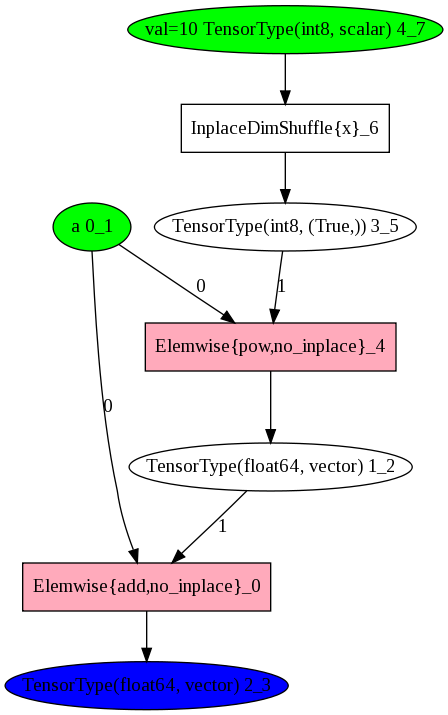
\includegraphics[width=0.35\textwidth]{pics/f_unoptimized.png}
\hspace{0.1\textwidth}
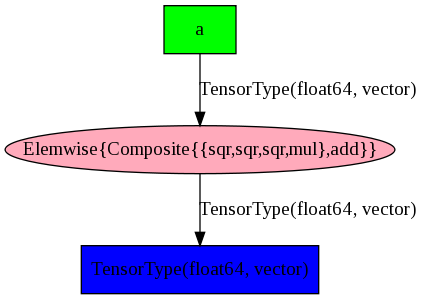
\includegraphics[width=0.35\textwidth]{pics/f_optimized.png}
\end{frame}


\begin{frame}{Overview of library}
  Theano is many things
  \begin{itemize}
  \item Language
  \item Compiler
  \item Python library
  \end{itemize}
\end{frame}

%\subsection{Operations}
%% \begin{frame}{Overview Language}
%%   Most of NumPy and more!
%%   \begin{itemize}
%%   \item Operations on scalars, vectors, matrices, tensors, and sparse variables
%%   \item Linear algebra
%%   \item Element-wise nonlinearities
%%   \item Convolution
%%   \item Indexing, slicing and advanced indexing.
%%   \item Reduction
%%   \item Dimshuffle (n-dim transpose)
%%   \end{itemize}
%% \end{frame}


\begin{frame}[fragile]
  \frametitle{Scalar math}
Some example of scalar operations:
\lstset{language=Python,
        commentstyle=\itshape\color{blue},
        stringstyle=\color{violet},
        }
\begin{lstlisting}
import theano
from theano import tensor as T
x = T.scalar()
y = T.scalar()
z = x + y
w = z * x
a = T.sqrt(w)
b = T.exp(a)
c = a ** b
d = T.log(c)
\end{lstlisting}
\end{frame}

\begin{frame}[fragile]
  \frametitle{Vector math}

\lstset{language=Python,
        commentstyle=\itshape\color{blue},
        stringstyle=\color{violet},
        }
\begin{lstlisting}
from theano import tensor as T
x = T.vector()
y = T.vector()
# Scalar math applied elementwise
a = x * y
# Vector dot product
b = T.dot(x, y)
# Broadcasting (as NumPy, very powerful)
c = a + b
\end{lstlisting}
\end{frame}

\begin{frame}[fragile]
  \frametitle{Matrix math}

\lstset{language=Python,
        commentstyle=\itshape\color{blue},
        stringstyle=\color{violet},
        }
\begin{lstlisting}
from theano import tensor as T
x = T.matrix()
y = T.matrix()
a = T.vector()
# Matrix-matrix product
b = T.dot(x, y)
# Matrix-vector product
c = T.dot(x, a)
\end{lstlisting}
\end{frame}

\begin{frame}[fragile]
  \frametitle{Tensors}
  Using Theano:
  \begin{itemize}
  \item Dimensionality defined by length of ``broadcastable'' argument
  \item Can add (or do other elemwise op) two
    tensors with same dimensionality
  \item Duplicate tensors along broadcastable axes to make size match
  \end{itemize}
\lstset{language=Python,
        commentstyle=\itshape\color{blue},
        stringstyle=\color{violet},
        }
\begin{lstlisting}
from theano import tensor as T
tensor3 = T.TensorType(
    broadcastable=(False, False, False),
    dtype='float32')
x = T.tensor3()
\end{lstlisting}
\end{frame}

\begin{frame}[fragile]
  \frametitle{Reductions}
\lstset{language=Python,
        commentstyle=\itshape\color{gray},
        stringstyle=\color{gray},
        keywordstyle=\color{gray},
        rulecolor=\color{gray},
        identifierstyle=\color{gray},
        basicstyle=\color{gray},
        }
\begin{lstlisting}
from theano import tensor as T
tensor3 = T.TensorType(
    broadcastable=(False, False, False),
    dtype='float32')
x = tensor3()
\end{lstlisting}

\lstset{language=Python,
        commentstyle=\itshape\color{blue},
        stringstyle=\color{violet},
        keywordstyle=\color{black},
        rulecolor=\color{black},
        identifierstyle=\color{black},
        basicstyle=\color{black},
        }
\begin{lstlisting}
total = x.sum()
marginals = x.sum(axis=(0, 2))
mx = x.max(axis=1)
\end{lstlisting}
\end{frame}

\begin{frame}[fragile]
  \frametitle{Dimshuffle}

\lstset{language=Python,
        commentstyle=\itshape\color{gray},
        stringstyle=\color{gray},
        keywordstyle=\color{gray},
        rulecolor=\color{gray},
        identifierstyle=\color{gray},
        basicstyle=\color{gray},
        }
\begin{lstlisting}
from theano import tensor as T
tensor3 = T.TensorType(
    broadcastable=(False, False, False))
x = tensor3()
\end{lstlisting}
\lstset{language=Python,
        commentstyle=\itshape\color{blue},
        stringstyle=\color{violet},
        keywordstyle=\color{black},
        rulecolor=\color{black},
        identifierstyle=\color{black},
        basicstyle=\color{black},
        }
\begin{lstlisting}
y = x.dimshuffle((2, 1, 0))
a = T.matrix()

b = a.T
# Same as b
c = a.dimshuffle((0, 1))

# Adding to larger tensor
d = a.dimshuffle((0, 1, 'x'))
e = a + d
\end{lstlisting}
\end{frame}

\begin{frame}[fragile]
  \frametitle{Indexing}
  As NumPy!
  This mean slices and index selection return view
\lstset{language=Python,
        commentstyle=\itshape\color{blue},
        stringstyle=\color{violet},
        }
\begin{lstlisting}
# return views, supported on GPU
a_tensor[int]
a_tensor[int, int]
a_tensor[start:stop:step, start:stop:step]
a_tensor[::-1] # reverse the first dimension

# Advanced indexing, return copy
a_tensor[an_index_vector] # Supported on GPU
a_tensor[an_index_vector, an_index_vector]
a_tensor[int, an_index_vector]
a_tensor[an_index_tensor, ...]
\end{lstlisting}
\end{frame}

\subsection{Compiling/Running}
\begin{frame}{Compiling and running expression}
  \begin{itemize}
  \item theano.function
  \item shared variables and updates
  \item compilation modes
%  \item TODO: optimizations
  \end{itemize}
\end{frame}

\begin{frame}[fragile]
  \frametitle{theano.function}

\lstset{language=Python,
        commentstyle=\itshape\color{blue},
        stringstyle=\color{violet},
        }
\begin{lstlisting}
>>> from theano import tensor as T
>>> x = T.scalar()
>>> y = T.scalar()
>>> from theano import function
>>> # first arg is list of SYMBOLIC inputs
>>> # second arg is SYMBOLIC output
>>> f = function([x, y], x + y)
>>> # Call it with NUMERICAL values
>>> # Get a NUMERICAL output
>>> f(1., 2.)
array(3.0)
\end{lstlisting}
\end{frame}

\begin{frame}{Shared variables}
  \begin{itemize}
  \item It’s hard to do much with purely functional programming
  \item ``shared variables'' add just a little bit of imperative programming
  \item A ``shared variable'' is a buffer that stores a numerical value for a Theano variable
  \item Can write to as many shared variables as you want, once each, at the end of the function
  \item Can modify value outside of Theano function with get\_value() and set\_value() methods.
  \end{itemize}
\end{frame}

\begin{frame}[fragile]
  \frametitle{Shared variable example}

\lstset{language=Python,
        commentstyle=\itshape\color{blue},
        stringstyle=\color{violet},
        }
\begin{lstlisting}
>>> from theano import shared
>>> x = shared(0.)
>>> updates = [(x, x + 1)]
>>> f = function([], updates=updates)
>>> f()
>>> x.get_value()
1.0
>>> x.set_value(100.)
>>> f()
>>> x.get_value()
101.0
\end{lstlisting}
\end{frame}


%% \begin{frame}{Which dict?}
%%   \begin{itemize}
%%   \item Use theano.compat.python2x.OrderedDict
%%   \item Not collections.OrderedDict
%%   \begin{itemize}
%%   \item This isn’t available in older versions of python
%%   \end{itemize}
%%   \item Not \{\} aka dict
%%   \begin{itemize}
%%   \item The iteration order of this built-in class is not
%%     deterministic (thanks, Python!) so if Theano
%%     accepted this, the same script could compile
%%     different C programs each time you run it
%%   \end{itemize}
%%   \end{itemize}
%% \end{frame}

\begin{frame}{Compilation modes}
  \begin{itemize}
  \item Can compile in different modes to get different kinds of programs
  \item Can specify these modes very precisely with arguments to theano.function
  \item Can use a few quick presets with environment variable flags
  \end{itemize}
\end{frame}

\begin{frame}{Interresting compilation configuration}
  Some Theano flags:
  \begin{itemize}
  \item mode=FAST\_RUN: default. Fastest execution, slowest compilation
  \item mode=FAST\_COMPILE: Fastest compilation, slowest execution. No C code.
  \item mode=DEBUG\_MODE: Adds lots of checks.
  \item optimizer=fast\_compile: mode=FAST\_COMPILE with C code.
  \item optimizer=stabilize: optimizer=fast\_compile with stability optimization.
  \end{itemize}
\end{frame}

\begin{frame}{Theano flags}
  Can be set globally:
  \begin{itemize}
  \item In a configuration file \~/.theanorc
  \item THEANO\_FLAGS=mode=FAST\_COMPILE python script.py
  \end{itemize}

  Sometimes as parameter of functions:
  \begin{itemize}
  \item theano.function(..., mode=``FAST\_COMPILE'')
  \end{itemize}
\end{frame}

\subsection{Modifying expressions}
\begin{frame}{Modifying expressions}
  There are ``macro'' that automatically build bigger graph for you.
  \begin{itemize}
  \item theano.grad
  \item Others
  \end{itemize}
  Those functions can get called many times, for example to get the 2nd
  derivative.
\end{frame}

\begin{frame}[fragile]
  \frametitle{The grad method}

\lstset{language=Python,
        commentstyle=\itshape\color{blue},
        stringstyle=\color{violet},
        }
\begin{lstlisting}
>>> x = T.scalar('x')
>>> y = 2. * x
>>> g = T.grad(y, x)
# Print the not optimized graph
>>> theano.printing.pydotprint(g)
\end{lstlisting}
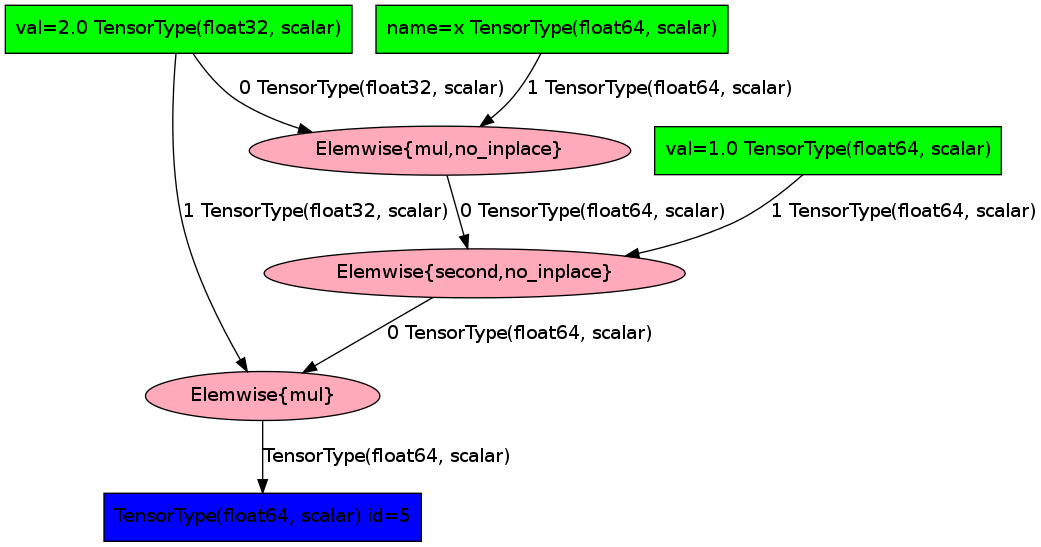
\includegraphics[width=0.75\textwidth]{pics/theano_grad.png}
\end{frame}

\begin{frame}[fragile]
  \frametitle{The grad method}
\lstset{language=Python,
        commentstyle=\itshape\color{gray},
        stringstyle=\color{gray},
        keywordstyle=\color{gray},
        rulecolor=\color{gray},
        identifierstyle=\color{gray},
        basicstyle=\color{gray},
        }
\begin{lstlisting}
>>> x = T.scalar('x')
>>> y = 2. * x
>>> g = T.grad(y, x)
\end{lstlisting}
\lstset{language=Python,
        commentstyle=\itshape\color{blue},
        stringstyle=\color{violet},
        keywordstyle=\color{black},
        rulecolor=\color{black},
        identifierstyle=\color{black},
        basicstyle=\color{black},
        }
\begin{lstlisting}
# Print the optimized graph
>>> f = theano.function([x], g)
>>> theano.printing.pydotprint(f)
\end{lstlisting}
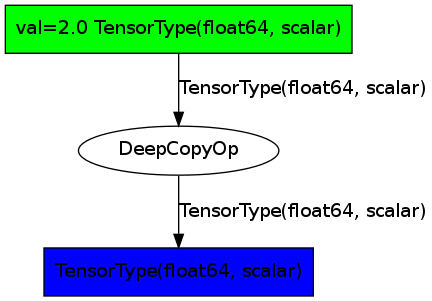
\includegraphics[width=0.4\textwidth]{pics/theano_grad_opt.png}
\end{frame}

\begin{frame}{Others}
  \begin{itemize}
  \item R\_op, L\_op for Hessian Free Optimization
  \item hessian
  \item jacobian
  \item clone the graph with replacement
  \item you can navigate the graph if you need
      (go from the result of computation to its input, recursively)
  \end{itemize}
\end{frame}

\subsection{GPU}
\begin{frame}{Enabling GPU}
  \begin{itemize}
  \item libgpuarray (new-backend) supports all dtype
    \begin{itemize}
    \item including float16 for storage
    \end{itemize}
  \item Theano's old GPU back-end removed from the master of Theano
  \item CUDA supports float64, but it is slow on gamer GPUs
  \end{itemize}
\end{frame}


\begin{frame}{CuDNN}
  \begin{itemize}
  \item V5 and V5.1 are supported
  \item V6 compile
  \item It is enabled automatically if available
  \item Theano flag to get an error if can't be used: ``dnn.enabled=True''
  \item Theano flag to disable it: ``dnn.enabled=False''
  \end{itemize}
\end{frame}


\begin{frame}{GPU: Theano flags}
  Theano flags allow to configure Theano. Can be set via a
  configuration file or an environment variable.

  To enable GPU:
  \begin{itemize}
  \item Set ``device=cuda'' (or a specific GPU, like ``cuda0'')
  \item Set ``floatX=float32''
  \item Optional: warn\_float64=\{'ignore', 'warn', 'raise', 'pdb'\}
  \item Instead of Theano flags, user can call ``theano.gpuarray.use('cuda0')''
  \end{itemize}
\end{frame}


\begin{frame}{floatX}
  Allow to change the dtype between float32 and float64.
  \begin{itemize}
  \item T.fscalar, T.fvector, T.fmatrix are all 32 bit
  \item T.dscalar, T.dvector, T.dmatrix are all 64 bit
  \item T.scalar, T.vector, T.matrix resolve to floatX
  \item floatX is float64 by default, set it to float32 for GPU
  \end{itemize}
\end{frame}

\subsection{Debugging}
\begin{frame}{Debugging}
  \begin{itemize}
  \item DebugMode: a mode that tests many things done by Theano (very slow)
  \item NanGuardMode: a mode that help find the cause of nan in the graph
  \item Error message
  \item theano.printing.debugprint: print a textual representation of computation
  \item profiling: To help know where time is spend
  \end{itemize}
\end{frame}

\begin{frame}[fragile]
  \frametitle{Error message: code}
\lstset{language=Python,
        commentstyle=\itshape\color{blue},
        stringstyle=\color{violet},
        }
\begin{lstlisting}
import numpy as np
import theano
import theano.tensor as T
x = T.vector()
y = T.vector()
z = x + x
z = z + y
f = theano.function([x, y], z)
f(np.ones((2,)), np.ones((3,)))
\end{lstlisting}
\end{frame}

\begin{frame}[fragile]
  \frametitle{Error message: 1st part}

\lstset{language=Python,
        commentstyle=\itshape\color{blue},
        stringstyle=\color{violet},
        basicstyle=\scriptsize
        }
\begin{lstlisting}
Traceback (most recent call last):
[...]
ValueError: Input dimension mis-match.
    (input[0].shape[0] = 3, input[1].shape[0] = 2)
Apply node that caused the error:
   Elemwise{add,no_inplace}(<TensorType(float64, vector)>,
                            <TensorType(float64, vector)>,
                            <TensorType(float64, vector)>)
Inputs types: [TensorType(float64, vector),
               TensorType(float64, vector),
               TensorType(float64, vector)]
Inputs shapes: [(3,), (2,), (2,)]
Inputs strides: [(8,), (8,), (8,)]
Inputs values: [array([ 1.,  1.,  1.]),
                array([ 1.,  1.]),
                array([ 1.,  1.])]
Outputs clients: [['output']]
\end{lstlisting}
\end{frame}

\begin{frame}[fragile]
  \frametitle{Error message: 2st part}
HINT: Re-running with most Theano optimization
disabled could give you a back-traces when this
node was created. This can be done with by setting
the Theano flags ``optimizer=fast\_compile''. If that does not
work, Theano optimizations can be disabled with
``optimizer=None''.\newline
HINT: Use the Theano flag ``exception\_verbosity=high''
for a debugprint of this apply node.
\end{frame}


\begin{frame}[fragile]
  \frametitle{Error message: traceback}

\lstset{language=Python,
        commentstyle=\itshape\color{blue},
        stringstyle=\color{violet},
        basicstyle=\footnotesize,
        xleftmargin=-1em
        }
\begin{lstlisting}
Traceback (most recent call last):
  File "test.py", line 9, in <module>
    f(np.ones((2,)), np.ones((3,)))
  File "/u/bastienf/repos/theano/compile/function_module.py",
       line 589, in __call__
    self.fn.thunks[self.fn.position_of_error])
  File "/u/bastienf/repos/theano/compile/function_module.py",
       line 579, in __call__
    outputs = self.fn()
\end{lstlisting}
\end{frame}


\begin{frame}[fragile]
  \frametitle{Error message: optimizer=fast\_compile}

\lstset{language=Python,
        commentstyle=\itshape\color{blue},
        stringstyle=\color{violet},
        }
\begin{lstlisting}
Backtrace when the node is created:
  File "test.py", line 7, in <module>
    z = z + y

\end{lstlisting}
\end{frame}


\begin{frame}[fragile]
  \frametitle{debugprint}

\lstset{language=Python,
        commentstyle=\itshape\color{blue},
        stringstyle=\color{violet},
        }
\begin{lstlisting}
>>> from theano.printing import debugprint
>>> debugprint(a)
Elemwise{mul,no_inplace} [id A] ''
 |TensorConstant{2.0} [id B]
 |Elemwise{add,no_inplace} [id C] 'z'
   |<TensorType(float64, scalar)> [id D]
   |<TensorType(float64, scalar)> [id E]
\end{lstlisting}
\end{frame}

%% \begin{frame}{Pylearn2}

%%   Machine Learning library aimed at researchers

%%   \begin{itemize}
%%     \item Built on top of Theano, for fast execution and use of GPU
%%     \item Easy to try variants of implemented algorithms, and to extend them (using Theano)
%%     \item Very modular, each component of the library can be used in isolation
%%     \item Experiments can be specified through a YAML config file, or by a Python script
%%     \item Scripts for visualizing weights, plot monitored values
%%   \end{itemize}
%% \end{frame}


%% \begin{frame}{libgpuarray}
%%   Goal: A common GPU $n$-dimensional array that can be reused by all projects, support for both CUDA and OpenCL.
%%   \newline \newline
%%   Motivation:
%%   \begin{itemize}
%%   \item Currently there are at least 6 different GPU arrays in Python
%%     \begin{itemize}
%%     \item CudaNdarray (Theano), GPUArray (pycuda), CUDAMatrix (cudamat), GPUArray (pyopencl), Clyther, Copperhead, ...
%%     \item There are even more if we include other languages.
%%     \end{itemize}
%%   \item They are incompatible
%%     \begin{itemize}
%%     \item None have the same properties and interface
%%     \end{itemize}
%%   \item All of them implement a subset of numpy.ndarray properties
%%   \item This is the new GPU backend on Theano
%%   \end{itemize}
%% \end{frame}


%% \begin{frame}{Project status?}
%%   \begin{itemize}
%%   \item Usable directly, but not all implementation available.
%%   \item Multiple GPUs works.
%%   \item Is the next GPU array container for Theano and is working.
%%     \begin{itemize}
%%     \item Not all Theano implementations available now.
%%     \item OpenCL misses more implementations.
%%     \item Multiple GPUs: supported in libgpuarray
%%     \item Multiple GPUs: close to get integrated in Theano.
%%     \end{itemize}
%%   \item Web site: \url{http://deeplearning.net/software/libgpuarray/}
%%   \end{itemize}
%% \end{frame}

%% \section{libgpuarray}
%% \begin{frame}
%%   \tableofcontents[currentsection]
%% \end{frame}
%% %TODO, make much shorter
%% \begin{frame}{libgpuarray: Design Goals}
%%   \begin{itemize}
%%   \item Have the base object in C to allow collaboration with more projects.
%%     \begin{itemize}
%%     \item We want people from C, C++, ruby, R, \ldots all use the same base GPU ndarray.
%%     \end{itemize}
%%   \item Be compatible with CUDA and OpenCL.
%%   \item Not too simple, (don’t support just matrix).
%%   \item Support all dtype.
%%   \item Allow strided views.
%%   \item But still easy to develop new code that support only a few memory layout.
%%     \begin{itemize}
%%     \item This ease the development of new code.
%%     \end{itemize}
%%   \end{itemize}
%% \end{frame}


\section{Models}
\subsection{Logistic Regression}
\begin{frame}
  \tableofcontents[currentsection]
\end{frame}


\begin{frame}[fragile]
  \frametitle{Inputs}
\lstset{language=Python,
        commentstyle=\itshape\color{blue},
        stringstyle=\color{violet},
        }
\begin{lstlisting}
# Load from disk and put in shared variable.
datasets = load_data(dataset)
train_set_x, train_set_y = datasets[0]
valid_set_x, valid_set_y = datasets[1]

# allocate symbolic variables for the data
index = T.lscalar()  # index to a [mini]batch

# generate symbolic variables for input minibatch
x = T.matrix('x')  # data, 1 row per image
y = T.ivector('y')  # labels
\end{lstlisting}
\end{frame}


\begin{frame}[fragile]
  \frametitle{Model}
\lstset{language=Python,
        commentstyle=\itshape\color{blue},
        stringstyle=\color{violet},
        }
\begin{lstlisting}
n_in = 28 * 28
n_out = 10

# weights
W = theano.shared(
        numpy.zeros((n_in, n_out),
                    dtype=theano.config.floatX))

# bias
b = theano.shared(
        numpy.zeros((n_out,),
                    dtype=theano.config.floatX))
\end{lstlisting}
\end{frame}


\begin{frame}[fragile]
  \frametitle{Computation}
\lstset{language=Python,
        commentstyle=\itshape\color{blue},
        stringstyle=\color{violet},
        }
\begin{lstlisting}
# the forward pass
p_y_given_x = T.nnet.softmax(T.dot(input, W) + b)

# cost we minimize: the negative log likelihood
l = T.log(p_y_given_x)
cost = -T.mean(l[T.arange(y.shape[0]), y])

# the error
y_pred = T.argmax(p_y_given_x, axis=1)
err = T.mean(T.neq(y_pred, y))
\end{lstlisting}
\end{frame}


\begin{frame}[fragile]
  \frametitle{Gradient and updates}
\lstset{language=Python,
        commentstyle=\itshape\color{blue},
        stringstyle=\color{violet},
        }
\begin{lstlisting}
# compute the gradient of cost
g_W, g_b = T.grad(cost=cost, wrt=(W, b))

# model parameters updates rules
updates = [(W, W - learning_rate * g_W),
           (b, b - learning_rate * g_b)]
\end{lstlisting}
\end{frame}


\begin{frame}[fragile]
  \frametitle{Training function}
\lstset{language=Python,
        commentstyle=\itshape\color{blue},
        stringstyle=\color{violet},
        }
\begin{lstlisting}
# compile a Theano function that train the model
train_model = theano.function(
    inputs=[index], outputs=(cost, err),
    updates=updates,
    givens={
        x: train_set_x[index * batch_size:
                       (index + 1) * batch_size],
        y: train_set_y[index * batch_size:
                       (index + 1) * batch_size]
    }
)
\end{lstlisting}
\end{frame}


\subsection{Convolution}
\begin{frame}
  \tableofcontents[currentsection]
\end{frame}
\begin{frame}[fragile]
  \frametitle{Inputs}
\lstset{language=Python,
        commentstyle=\itshape\color{blue},
        stringstyle=\color{violet},
        }
\begin{lstlisting}
# Load from disk and put in shared variable.
datasets = load_data(dataset)
train_set_x, train_set_y = datasets[0]
valid_set_x, valid_set_y = datasets[1]

# allocate symbolic variables for the data
index = T.lscalar()  # index to a [mini]batch

x = T.matrix('x')   # the data, 1 row per image
y = T.ivector('y')  # labels

# Reshape matrix of shape (batch_size, 28 * 28)
# to a 4D tensor, compatible for convolution
layer0_input = x.reshape((batch_size, 1, 28, 28))
\end{lstlisting}
\end{frame}


\begin{frame}[fragile]
  \frametitle{Model}
\lstset{language=Python,
        commentstyle=\itshape\color{blue},
        stringstyle=\color{violet},
        }
\begin{lstlisting}
image_shape=(batch_size, 1, 28, 28)
filter_shape=(nkerns[0], 1, 5, 5)

W_bound = ...
W = theano.shared(
    numpy.asarray(
        rng.uniform(low=-W_bound, high=W_bound,
                    size=filter_shape),
        dtype=theano.config.floatX))

# the bias is a 1D tensor
# one bias per output feature map
b_values = numpy.zeros((filter_shape[0],),dtype=...
b = theano.shared(b_values)
\end{lstlisting}
\end{frame}


\begin{frame}[fragile]
  \frametitle{Computation}
\lstset{language=Python,
        commentstyle=\itshape\color{blue},
        stringstyle=\color{violet},
        }
\begin{lstlisting}
# convolve input feature maps with filters
conv_out = nnet.conv2d(input=x, filters=W)

# pool each feature map individually,
# using maxpooling
pooled_out = pool.pool_2d(
    input=conv_out,
    ds=(2, 2),  // poolsize
    ignore_border=True)

output = T.tanh(pooled_out +
                b.dimshuffle('x', 0, 'x', 'x'))
\end{lstlisting}
\end{frame}


\iffalse
\subsection{Scan}
\begin{frame}
  \frametitle{Scan}
\begin{itemize}
\item Allows looping (for, map, while)
\item Allows recursion (reduce)
\item Allows recursion with dependency on many of the previous time steps
\item Optimize some cases like moving computation outside of scan
\item The Scan grad is done via Backpropagation Through Time(BPTT)
\end{itemize}
\end{frame}

\begin{frame}{When not to use scan}
\begin{itemize}
\item If you only need it for ``vectorization'' or
  ``broadcasting''. tensor and numpy.ndarray support them
  natively. This will be much better for that use case.

\item If you do a fixed number of iteration that is very small (2,3). You
  are probably better to just unroll the graph to do it.

\end{itemize}
\end{frame}


\begin{frame}[fragile,allowframebreaks]
  \frametitle{Scan Example1: Computing tanh(v.dot(W) + b) * d where d is binomial}

\lstset{language=Python,
        commentstyle=\itshape\color{blue},
        stringstyle=\color{violet},
        basicstyle=\footnotesize
        }
\begin{lstlisting}
import theano
import theano.tensor as T
import numpy as np

# define tensor variables
W = T.matrix("W")
X = T.matrix("X")
b_sym = T.vector("b_sym")

# define shared random stream
trng = T.shared_randomstreams.RandomStreams(1234)
d=trng.binomial(size=W[1].shape)
\end{lstlisting}
\end{frame}


\begin{frame}[fragile]
  \frametitle{Scan Example1: Computing tanh(v.dot(W) + b) * d where d is binomial (2)}

\lstset{language=Python,
        commentstyle=\itshape\color{blue},
        stringstyle=\color{violet},
        }
\begin{lstlisting}
results, updates = theano.scan(
    lambda v: T.tanh(T.dot(v, W) + b_sym) * d,
    sequences=X)
f = theano.function(inputs=[X, W, b_sym],
                    outputs=[results],
                    updates=updates)
x = np.eye(10, 2, dtype=theano.config.floatX)
w = np.ones((2, 2), dtype=theano.config.floatX)
b = np.ones((2), dtype=theano.config.floatX)

print f(x, w, b)
\end{lstlisting}
\end{frame}

\begin{frame}[fragile]
  \frametitle{Scan Example2: Computing pow(A, k)}

\lstset{language=Python,
        commentstyle=\itshape\color{blue},
        stringstyle=\color{violet},
        }
\begin{lstlisting}
import theano
import theano.tensor as T
theano.config.warn.subtensor_merge_bug = False

k = T.iscalar("k")
A = T.vector("A")

def inner_fct(prior_result, B):
    return prior_result * B
\end{lstlisting}
\end{frame}

\begin{frame}[fragile]
  \frametitle{Scan Example2: Computing pow(A, k) (2)}

\lstset{language=Python,
        commentstyle=\itshape\color{blue},
        stringstyle=\color{violet},
        }
\begin{lstlisting}
result, updates = theano.scan(
    fn=inner_fct,
    outputs_info=T.ones_like(A),
    non_sequences=A, n_steps=k)

# Scan provides us with A ** 1 through A ** k.
# Keep only the last value. Scan optimizes memory.
final = result[-1]

power = theano.function(inputs=[A, k], outputs=final,
                      updates=updates)
print power(range(10), 2)
#[  0.   1.   4.   9.  16.  25.  36.  49.  64.  81.]
\end{lstlisting}
\end{frame}

\begin{frame}[fragile]
  \frametitle{Scan signature}

\lstset{language=Python,
        commentstyle=\itshape\color{blue},
        stringstyle=\color{violet},
        }
\begin{lstlisting}
result, updates = theano.scan(
    fn=inner_fct,
    sequences=[]
    outputs_info=[T.ones_like(A)],
    non_sequences=A,
    n_steps=k)
\end{lstlisting}

\begin{itemize}
\item Updates are needed if there are random numbers generated in the inner function
\begin{itemize}
\item Pass them to the call theano.function(..., updates=updates)
\end{itemize}
\item The inner function of scan takes arguments like this:
   scan: sequences, outputs\_info, non sequences
\end{itemize}

\end{frame}
\fi

\section{Lasagne}
\begin{frame}
  \tableofcontents[currentsection]
\end{frame}

\begin{frame}{What is Lasagne}
  Lasagne is a thin framework/library on top of Theano.
  http://lasagne.readthedocs.org/
  \begin{itemize}
  \item Does not hide Theano
  \item Easily build Theano graphs by using layers
  \item Contains many preimplemented losses and optimizers
  \item Does not include a training loop
  \end{itemize}
\end{frame}


\begin{frame}[fragile]
  \frametitle{Lasagne MLP Example: Input Variables}

\lstset{language=Python,
        commentstyle=\itshape\color{blue},
        stringstyle=\color{violet},
        }
\begin{lstlisting}
  input_var = T.tensor4('inputs')
  target_var = T.ivector('targets')
\end{lstlisting}
\end{frame}

\begin{frame}[fragile]
  \frametitle{Lasagne MLP Example: Model}

\lstset{language=Python,
        commentstyle=\itshape\color{blue},
        stringstyle=\color{violet},
        }
\begin{lstlisting}
# Input and dropout layer
net = lasagne.layers.InputLayer(
    shape=(None, 1, 28, 28), input_var=input_var)
net = lasagne.layers.DropoutLayer(net, p=0.2)
# Hidden layers and dropout:
nonlin = lasagne.nonlinearities.rectify
for _ in range(2):
    net = lasagne.layers.DenseLayer(
        network, 800, nonlinearity=nonlin)
    net = lasagne.layers.dropout(network, p=0.5)
# Output layer:
softmax = lasagne.nonlinearities.softmax
net = lasagne.layers.DenseLayer(network, 10,
    nonlinearity=softmax)
\end{lstlisting}
\end{frame}

\begin{frame}[fragile]
  \frametitle{Lasagne MLP Example: Train Function}

\lstset{language=Python,
        commentstyle=\itshape\color{blue},
        stringstyle=\color{violet},
        }
\begin{lstlisting}
pred = lasagne.layers.get_output(network)
cat_cross_ent = lasagne.objectives.
    categorical_crossentropy
loss = cat_cross_ent(pred, target_var)
loss = loss.mean()

params = lasagne.layers.get_all_params(
    network, trainable=True)
updates = lasagne.updates.nesterov_momentum(
    loss, params, learning_rate=0.01,
    momentum=0.9)

train_fn = theano.function([input_var, target_var],
                           loss, updates=updates)
\end{lstlisting}
\end{frame}

\begin{frame}[fragile]
  \frametitle{Lasagne MLP Example: Test Function}

  \lstset{language=Python,
          commentstyle=\itshape\color{blue},
          stringstyle=\color{violet},
   }
  \begin{lstlisting}
test_pred = lasagne.layers.get_output(
    network, deterministic=True)
test_loss = cat_cross_ent(test_pred, target_var)
test_loss = test_loss.mean()

test_acc = T.mean(T.eq(T.argmax(test_pred, axis=1),
                       target_var),
                  dtype=theano.config.floatX)

val_fn = theano.function([input_var, target_var],
                         [test_loss, test_acc])
\end{lstlisting}
\end{frame}

\section{Exercises}
\begin{frame}
  \tableofcontents[currentsection]
\end{frame}

\begin{frame}{ipython notebook}
\begin{itemize}
\item Introduction
\item Exercises (Theano only exercises)
\item LeNet (small CNN model to quickly try it)
\item Reuse VGG16 features: reuse VGG16 features to do classification of 2 new classes
\end{itemize}
\end{frame}


\section{End}
\begin{frame}{Further hands-on training}
Check out the Self-Paced labs at the conference:
\begin{itemize}
  \item Deep Learning, CUDA, OpenACC, Tools and more!
  \item Just grab a seat and take any available lab
  \item \underline{Located in the lower-level outside of LL20C}\newline
\end{itemize}

You will also receive Credits to take additional labs at nvidia.qwiklab.com
\begin{itemize}
\item Log in using the same account you used in this lab
\end{itemize}
\end{frame}

\begin{frame}{Where to learn more}
\normalsize
\begin{itemize}
\item Deep Learning Tutorials with Theano: \url{deeplearning.net/tutorial}
\item Theano tutorial: \url{deeplearning.net/software/tutorial}
\item Theano website: \url{deeplearning.net/software}
\item Lasagne documentation: http://lasagne.readthedocs.io/
\item You can also see frameworks on top of Theano like Blocks, Keras, Lasagne, ...
\end{itemize}

\end{frame}

\begin{frame}{Questions, acknowledgments}
\Huge
\begin{center}
Questions?\newline
Acknowledgments
\end{center}
\normalsize
\begin{itemize}
\item All people working or having worked at the MILA institute
\item All Theano users/contributors
\item Compute Canada, RQCHP, NSERC, NVIDIA, and Canada Research Chairs for providing funds, access to computing resources, hardware or GPU libraries.
\end{itemize}

\end{frame}


\end{document}
